\subsection{User guide}
The user guide is divided into the two following parts, A) Android application (Client) and B) Java applikation (Server)

\subsubsection{Android application (Client)}
There is a user interface (UI) for the client, which is sketched at the following figure.

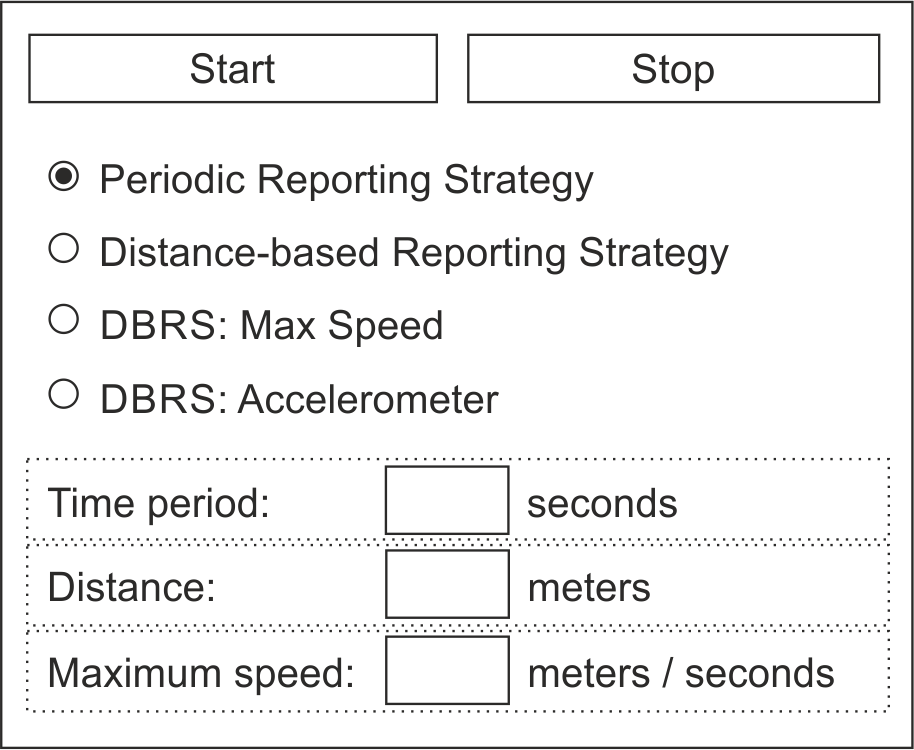
\includegraphics{GUI}

Chose one of the four algorithms, set the respective settings and press the "Start" button. Then the client sends locations to the server according to the chosen algorithm.

The server is expected to be located at www.rohdef.dk at port 57005, which is defined at line 37 in the class ServerRegistrar (Package: dk.au.cs.EagleEye2.registrars).

\subsubsection{Java applikation (Server)}
There is no GUI for the server, but it takes the following command line arguments.

\begin{itemize} \itemsep1pt \parskip0pt \parsep0pt
  \item runServer: Listen for a client to send locations
  \item parseKML: Parse the saved locations to KML.
  \item testMode: Return the text capitalized to the client.
\end{itemize}

The server listens at port 57005, which is defined at line 76 in the class Main.